\documentclass[a4paper,oneside]{book}

% Egy hasznos Mac OS X-es videó:
% http://www.youtube.com/watch?v=XFiLjB9UNaA&feature=related

% Oyepa, Working Tagged Filesystem:
% http://pages.stern.nyu.edu/~marriaga/software/oyepa/

\usepackage{diplomamunka}

\usepackage{listings}
\usepackage{tikz}

\usepackage{rotating}

\usepackage{color}
\definecolor{comment}{rgb}{0,0.6,0.2}

% Code colorature
\definecolor{paszt}{RGB}{252,252,252}
\definecolor{keret}{RGB}{220,220,220}
\lstset{
backgroundcolor=\color{paszt},
% showlines=true,
framexleftmargin=4mm,
framexrightmargin=4mm,
framextopmargin=2mm,
framexbottommargin=2mm,
frameround=tttt,
frame=trbl,
rulecolor=\color{keret},
extendedchars=true,
literate={á}{{\'a}}1 {é}{{\'e}}1 {ö}{{\"o}}1 {ő}{{\H{o}}}1 {ó}{{\'o}}1,
%inputencoding=utf8
}

% Line spacing (1.5-ös sorköz)
%\linespread{1.2}

% Set spacing in source code (normál sorköz -1.5)
%\lstset{
%lineskip={-3pt}
%}

\usepackage{pslatex}

%%% Font settings
% \usepackage{times}
\usepackage{lmodern} % !!!
% \usepackage{chancery}
% \usepackage{charter}
% \usepackage{palatino}
% \usepackage{mathpazo}
% \usepackage{mathpple} % !!!
% \usepackage{mathptmx}

\usepackage{pstricks}

\usepackage{java}
\usepackage{sql}

\begin{document}

% \pagestyle{empty} %a címlapon ne legyen semmi=empty, azaz nincs fejléc és lábléc

% Címlap
\begin{center}
\begin{tabular*}{\hsize}{@{}c@{\extracolsep{\fill}}c@{\extracolsep{\fill}}c@{}}
\multirow{2}[4]*{
\epsfig{file=images/ME_logo.eps,height=2truecm}}& \textcolor{blue}{\large\bfseries MISKOLCI EGYETEM}&\multirow{2}[4]*{
\epsfig{file=images/gepesz_logo.eps,height=1.6truecm}}\\
&\textcolor{blue}{\large\bfseries GÉPÉSZMÉRNÖKI ÉS INFORMATIKAI KAR}&\\
\end{tabular*}
\end{center}

\vglue 2.5truecm %függleges helykihagyás

\pagestyle{empty}

%A szakdolgozat címe, akár több sorban is
{\LARGE
\begin{center}
\textcolor{blue}{\Large\bfseries TDK DOLGOZAT}
\end{center}}

\vspace*{2.5truecm}
\begin{center}
% (Tag Based Document Management)
\LARGE\bfseries Lekérdezőnyelv és adatbáziskezelő rendszer \\
kétdimenziós térképadatok kezeléséhez
\end{center}
\vglue 2cm

{\large
\begin{center}
\begin{tabular}{c}
{\bfseries Kiss Viktor}\\
Gazdaságinformatikus BSc
\end{tabular}
\end{center}
\vglue 3cm
\begin{center}
\textbf{Konzulens:}
\end{center}
\medskip
\begin{center}
\begin{tabular}{ccc}
\textbf{Piller Imre} \\
tanársegéd \\
Alkalmazott Matematikai Intézeti Tanszék \\
\end{tabular}
\end{center}
\vfill
{\large

\begin{center}
\textbf{\textsc{Miskolc, 2016}}
\end{center}}

\newpage


% Font size
% \large

% Tartalomjegyzék
\tableofcontents
\thispagestyle{empty}
\cleardoublepage

% Set page style !!!
\pagestyle{fancy}

% Set number of page
\setcounter{page}{1}

% Chapters
\Chapter{Bevezetés}

Számos alkalmazásban (tipikusan például a számítógépes játékokban) szükség  van kétdimenziós térképek adatainak tárolására, és az azokon lévő entitások kezelésére. Ennek a megvalósítása az egyes implementációkban sok közös elemet tartalmaz. Az általam definiált lekérdezőnyelv, és a hozzá készített adatbázis kezelő rendszer eszközt biztosít a programozók számára, hogy a térképek elemeit, és az elemek attribútumait egyszerűbben, egy lekérdezőnyelvi interfészen keresztül érhessék el. A térképen lévő elemeket entitásoknak nevezzük. A nyelvben definiálhatjuk az entitások osztályait. Az adatbázismotor a gyakori műveletekhez nyelvi szintű támogatást ad. Megfogalmazhatunk például olyan lekérdezéseket, amelyekkel entitások ütközését, vagy az azok közötti távolságokat vizsgáljuk. Adatbázisról lévén szó a fejlesztőknek nem szükséges a térképadatok perzisztens tárolási módjával külön foglalkozniuk.
\Chapter{Domain specifikus lekérdezőnyelvek}

A DSL egy olyan nyelv, amely egy adott feladatkör problémáinak megoldására lett létrehozva. Magasabb absztrakciós szinten lehet vele a problémákat megfogalmazni.
Elrejt alacsony szintű műveleteket, például változók felszabadítása.

TODO: Ide azt kellene leírni, hogy
\begin{itemize}
\item Milyen más területeken van szükség még domain specifikus nyelvekre?

Beágyazott szkript nyelvek esetén beszélhetünk DSL nyelvről, ilyenkor valamilyen specializált feladat ellátását támogató kód készíthető a segítségével. Az SAP vállalatirányítási rendszerhez is készült DSL szkript nyelv. Az SAPScript az egy eszköz az SAP rendszeren belül, amely eszközt biztosít , hogy formokat tervezzünk, nyomtassunk, stb.

Geoinformatika: A földmérés, távérzékelés, földrajz és térképészet új módszereit és lehetőségeit kutató tudomány. A térinformatikai rendszerek alkalmazása nagyon széles. A geográfiai adatok kezeléséhez is létrehoztak DSL nyelveket. Vannak olyan adatbázisok, melyek kifejezetten térkép adatok tárolására, és azok kezelésére lettek tervezve.


\item A játékfejlesztésben milyen problémák vannak, amelyekre egy adatbázismotor megoldást tud adni?

Térképadatok mellett, az üzleti logika perzisztens tárolását is lehetővé teszi.

A játékfejlesztésben az ütközés vizsgálat megoldása amennyire fontos feladat, oly annyira nehéz is. Hogyan észleljük az ütközést és mi történjen ennek hatására?
Ezen problémákkal nem kell a játékfejlesztőnek foglalkoznia, ezeket nyelvi szinten szolgáltatásként igénybe vehetik az adatbázismotortól.

Az ütközésvizsgálat mellett az útvonal tervezés sem triviális feladat. Legrövidebb út meghatározása két pont között úgy, hogy közben a térképen lévő entitásokat kikerülje.

A térkép felépítése nem a programozó feladata, ő lekérdezésekkel létrehozhatja azt.

Entitások közötti távolság kiszámítása sem az üzleti logika fejlesztőinek feladata, az adatbázismotor elvégzi ezt is helyettük.



\item Hogyan integrálható be egy ilyen szoftverkomponens/szoftvereszköz a fejlesztési folyamatba?
1. Külső (external) DSL: Szintaktikája eltér a szoftver megírásához használt programozási nyelvétől. A külső DSL szintaktikája lehet saját fejlesztésű, vagy épülhet egy szabványos formátumra, például XML-re.
Példák: reguláris kifejezések, SQL.

2. Belső (internal) DSL: A befogadó nyelv egy kis részhalmazát használja, jellemzően a programozási eszközök egy szűk körére szorítkozik, vagy a nyelvet sajátos stílusban használja.
\end{itemize}
\Chapter{A lekérdezőnyelv}

\section{Az adatbázis szerkezete}

A lekérdezőnyelv bemutatása előtt érdemes megnézni, hogy az adatbázis hogyan épül fel, és a nyelv egyes funkciói milyen gyakorlati problémákat oldanak meg. Ehhez a következő fogalmak tisztázására van szükségünk.
\begin{itemize}
\item \textit{adatbázis}: Az adatbázis a kezelendő adatok legnagyobb logikai egységét jelenti. Ez tartalmaz térképeket, osztálydefiníciókat.
\item \textit{térkép}: Az objektum példányok adatbázishoz kötődnek.
\item \textit{osztály}: A tárolandó elemek szerkezetét (\textit{sémáját}) írják le az osztálydefiníciók. Az alaptípusok esetében azokat az adatbázis közvetlenül biztosítja. Osztályokat a felhasználók is definiálhatnak, amelyeket azt követően az alaptípusokhoz hasonlóan tudnak majd használni.
\item \textit{objektum}: Az osztályokból objektumokat példányosíthatunk, ha megadjuk az e\-gyes attribútumok értékeit. Ezek az objektum példányok az adott térképhez kötődnek.
\item \textit{réteg}: A térképeknek van egy saját, lazább logikai felbontása, amely az objektumok egy diszjunkt csoportosítását adja. Azon objektumok, amelyek rendelkeznek pozícióval tartalmaznak még egy réteg azonosítót.
\item \textit{entitás}: Egy \texttt{Entity} alaptípusból létrehozott példány. Ezek azok, amelyek a térképen ténylegesen meg is fognak jelenni.
\end{itemize}

A lekérdezőnyelv bemutatására, az elemek funkcióinak definiálására ebben a fejezetben kerül sor. Az egyes lekérdezéstípusokhoz, és kifejezésekhez tartozó nyelvi diagramokat az implementációval foglalkozó fejezetben találjuk.

A következő szakaszok arra térnek ki, hogy a gyakorlatban előforduló gyakori problémákat milyen formában oldhatjuk meg a lekérdezőnyelv segítségével majd.

\subsection{Alkalmazáslogika kezelése}

Az adatbázisban tárolt elemekhez gyakran szükség lehet olyan további metaadatok megadására, amely az alkalmazáslogika kialakítása szempontjából lesz majd fontos. Ezeket a többletinformációkat saját osztályok definiálásával tudjuk megadni. Ez nagyon hasonló az SQL-ben a táblák sémájának definiálásához. Osztályok definiálási módjára a \texttt{CREATE} kifejezés bemutatásánál láthatunk majd példákat.

\subsection{Rétegkezelés}

Az adatbázis egy térképen belül rétegeket is értelmez. A térképek eredendően kétdimenziósak, ezzel viszont egy diszkrét, harmadik dimenziót is kapunk. Ez akkor lehet hasznos, amikor például ütközés vizsgálatnál a különböző szinteken lévő elemek ütközését külön-külön szeretnénk vizsgálni.

Két alapértelmezett attribútumot bevezetése volt szükség, úgy mint
\begin{itemize}
\item \texttt{zlayer}: A réteg azonosítószáma.
\item \texttt{zindex}: A rétegen belül egy sorszám, amely egyedi az objektumra nézve a rétegen belül.
\end{itemize}

A réteg és az index tehát az objektumot egyértelműen azonosítja. Ami miatt mégis szükség van az \texttt{id} azonosítóra, mert a réteg és az index is változtatható, ami egy azonosítónál nem szerencsés, illetve vannak nem réteghez kötött objektumok is.

Ha két elem más szinten van, akkor a \texttt{zlayer} attribútumuk értéke eltérő. Különböző rétegekben lévő objektumok között az ütközésvizsgálat nincs értelmezve.

A \texttt{zindex} attribútum megjelenítésnél a kirajzolási sorrend miatt érdekes. Mivel a rétegen belül nincs más sorrendi megkötés, ezért a takarási feladat csak így oldható meg.

Összefoglalva tehát minden objektumnak van \texttt{id}, \texttt{className}, \texttt{zlayer} és \texttt{zindex}.

\subsection{Térkép mentése és visszaállítása}

Az alkalmazások tipikusan a futtatások között is tárolják az adatokat. Az adatbázis használatának egyik nagy előnye, hogy így a program megírásánál a perzisztenciával már nem kell foglalkozni, mivel azt az adatbázis meg tudja oldani. Térképeket egyszerűen létre tudunk hozni, el tudjuk menteni benne az adatokat, illetve vissza tudjuk azokat tölteni.

\section{Alaptípusok}

A lekérdezőnyelv típusos. Tartalmaz előre definiált típusokat (\textit{alaptípusok}, \textit{gyári típusok}), illetve a nyelv lehetőséget ad új típusok definiálására is (\textit{felhasználói típusok}).

Az alaptípusok hierarchiáját \aref{fig:types} ábrán láthatjuk. Az élek itt tartalmazási kapcsolatot jelölnek. A nyelv csak kompozícióra ad lehetőséget.

A típusokból hasonlóképpen tudunk példányokat létrehozni, mint ahogy az objektum orientált programozási nyelvekben. A típus nevét követő zárójelekben adhatjuk meg a példány létrehozásához szükséges értékeket egy vesszővel elválasztott listában.

Minden objektumnak a típusa mellett van azonosítója is. Ezt az \texttt{id} attribútumában tárolja. Értéket példányosításkor automatikusan kap. Az objektumtól le tudjuk azt kérdezni, viszont változtatni nem lehet.

A következő szakaszokban az alaptípusok bemutatására kerül sor. A használati módjuk, paraméterezésük szemléltetéséhez már itt is lekérdezések szerepelnek, viszont azok részletes bemutatása majd csak a műveleti rész taglalásánál szerepel.

\begin{figure}[htb]
\begin{center}
    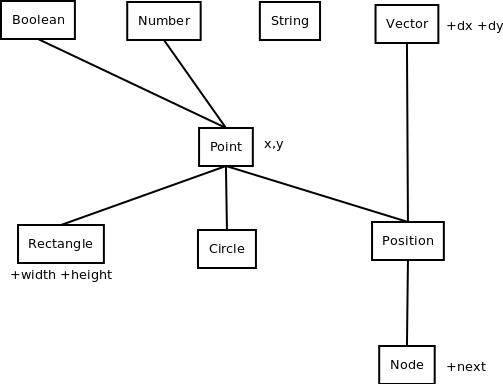
\includegraphics[scale=0.7]{images/types}
    \caption{A lekérdezőnyelv alaptípusai}
    \label{fig:types}
\end{center}
\end{figure}

\subsection{Boolean}

A \textit{Boolean} a nyelvben a logikai adattípus. Értéke \texttt{true} vagy \texttt{false} lehet. Paraméter nélküli létrehozás esetén az alapértelmezett értéke \texttt{false}. Az alábbi példákban az \texttt{azeroth} nevű térképre kerülnek beszúrásra logikai értékek.

\begin{sql}
INSERT Boolean INTO azeroth VALUES (true);
INSERT Boolean INTO azeroth VALUES (false);
INSERT Boolean INTO azerith VALUES (
    { SELECT bool FROM azeroth
      WHERE bool IS Boolean AND bool.id = 11 }
);
\end{sql}

Az utolsó példából látható, hogy a logikai típusú objektum is teljes értékű objektum, így az is rendelkezik azonosítóval (\texttt{id}).

\subsection{Number}

A \textit{Number} típus valós vagy egész szám 4 byteon való tárolására alkalmas. A lekérdezőnyelv nem különböztet meg előjeles és előjel nélküli változatot.

\begin{sql}
INSERT Number INTO azeroth VALUES (2);
INSERT Number INTO azeroth VALUES (
    { SELECT number FROM azeroth
      WHERE number IS Number AND number.id = 11 }
);
INSERT Number INTO azeroth VALUES (
    { SELECT number FROM azeroth
      WHERE number HAS x AND number.x IS Number AND number.id = 11 }
);
\end{sql}

\subsection{String}

Szöveges értékek tárolására a \textit{String} típust használhatjuk.

\begin{sql}
INSERT String INTO azeroth VALUES (alma);
INSERT String INTO azeroth VALUES (
    { SELECT string FROM azeroth
      WHERE string IS String AND string.id = 11 }
);
\end{sql}

\subsection{Point}

A térképen az elemek helyét pontok adják, amelyet \textit{Point} típusú objektumokban tárolhatunk. A pontnak sem kiterjedése, sem iránya nincs. Tulajdonképpen két \textit{Number} típusú értéket fog össze egy egységbe. A pont koordinátáit a geometriában használatos $(x, y)$ párral adhatjuk meg.

\begin{sql}
INSERT Point(x, y) INTO azeroth VALUES (10, 20);
INSERT Point(x, y) INTO azeroth VALUES (Number(10), 20);
INSERT Point(x, y) INTO azeroth VALUES (10, Number(20));
INSERT Point(x, y) INTO azeroth VALUES (
{ SELECT point FROM azeroth
  WHERE point IS Point AND point.id = 11 });
\end{sql}

Az utolsó beszúrás esetében egy másik \textit{Point} típusú objektumra hivatkozunk.

\noindent Amennyiben annak az értéke változik valamelyik a kettő közül, akkor ennek is változni fog.

\begin{sql}
INSERT Point(x, y) INTO azeroth VALUES ({
  SELECT number FROM azeroth
  WHERE number is Number AND number.id = 11 }, 10);
\end{sql}

Ilyenkor a pont \texttt{x} attribútuma egy másik \textit{Number} típusú objektumra mutat, tehát ha az változik, akkor a pont attribútuma is fog.

\begin{sql}
INSERT Point(x, y) INTO azeroth VALUES (
    { SELECT number FROM azeroth
    WHERE number is Number AND number.id = 11 },
    { SELECT number FROM azeroth
    WHERE number is Number AND number.id = 12 }
);
\end{sql}

Ebben mind a két attribútuma más \textit{Number} objektumra mutat.

\subsection{Vector}

A \textit{Vector} típus itt a geometriai értelemben véve irány tárolását teszi lehetővé. A ponthoz hasonlóan ez is két \textit{Number} értéket fog össze, ennek viszont csak iránya van, helye nincsen.

\begin{sql}
INSERT Vector(dx, dy) INTO azeroth VALUES (10, 20);
INSERT Vector(dx, dy) INTO azeroth VALUES (Number(10), Number(20));
INSERT Vector(dx, dy) INTO azeroth VALUES (Number(10), 20);
INSERT Vector(dx, dy) INTO azeroth VALUES (10, Number(20));
INSERT Vector(dx, dy) INTO azeroth VALUES (Vector(10, 20));
INSERT Vector(dx, dy) INTO azeroth VALUES (
{ SELECT vector FROM azeroth WHERE vector IS Vector AND vector.id = 11 }
);
\end{sql}

Ilyenkor egy másik \textit{Vector} objektumra hivatkozik, tehát ha annak az értéke változik valamelyik a kettő közül, akkor ennek is fog.

\begin{sql}
INSERT Vector(dx, dy) INTO azeroth VALUES (
{ SELECT number FROM azeroth
  WHERE number is Number AND number.id = 11 }, 10);
\end{sql}

Ilyenkor a vector \texttt{dx} attribútuma egy másik \textit{Number} objektumra mutat, tehát ha az változik, akkor ez is fog.

\begin{sql}
INSERT Vector(dx, dy) INTO azeroth VALUES (
    { SELECT number FROM azeroth
      WHERE number is Number AND number.id = 11 },
    { SELECT number FROM azeroth
      WHERE number is Number AND number.id = 12 }
);
\end{sql}

A ponthoz hasonlóan itt is megadható függetlenül a két \textit{Number} érték.


\subsection{Rectangle}

A \textit{Rectangle} típus téglalap adatainak tárolására szolgál. Tartalmaz egy pontot, amelyben tárolja a bal felső sarkának koordinátáit, illetve egy kiterjedést, amely a szélesség és magasság attribútumokat adja.

\begin{sql}
INSERT Rectangle(location(x, y), size(width, height)) INTO azeroth 
VALUES ((10, 10), (100, 200)); 
INSERT Rectangle(x, y, width, height) INTO azeroth
VALUES (10, 20, 30, 40);
\end{sql}

Itt az a lényeg, hogy lehet belül azzal a new nélküli kifejezéssel is visszaadatni új objektumot.

\subsection{Oval}

Az \textit{Oval} típus ovális alakzatok tárolását teszi lehetővé. 

\begin{sql}
INSERT Oval(x, y, width, height) INTO azeroth 
VALUES (10, 300, 12, 32);
\end{sql}

A fenti lekérdezés eredménye, hogy egy olyan oválist illeszt az "azeroth" nevű térképre, aminek a bal felső befoglaló téglalapjának a sarka a $(10, 300)$ pontra esik, a szélessége 12, a magassága 32. 

\subsection{Position}

A pozíciók leírásához használhatjuk a \textit{Position} osztályt. Ennek van helye és iránya. Lényegében egy pont és egy vektor objektumot fog össze egy logikai egységbe.

\begin{sql}
INSERT Position(location(x, y), direction(dx, dy)) INTO
azeroth VALUES ((10, 10), (100, 100));
INSERT Position(x, y, dx, dy) INTO azeroth VALUES (10, 10, 100, 100);
\end{sql}

A pozíciókat közvetlenül az attribútumok értékeivel, vagy pedig részlegesen a részobjektumaival is példányosíthatjuk.

\begin{sql}
INSERT Position(x, y, dx, dy) INTO azeroth VALUES (10, 10, 100, 200);
\end{sql}

Ebben az esetben a sorrend \texttt{x}, \texttt{y}, \texttt{dx} és \texttt{dy}. 


\subsection{Node}

A nyelv a dinamikus adatszerkezetek leírását láncolással oldja meg. Az alkalmazási területeket figyelembe véve általában pozíciók láncolására lehet szükség. A \textit{Node} típus egy pozíció típusú attribútumot és egy hivatkozást tartalmaz a következő \textit{Node} objektumra. Ennek a segítségével megadhatunk útvonalakat, fákat vagy általános irányított gráfokat.

\begin{sql}
INSERT Node(x, y, dx, dy, next, isFirst) INTO 
azeroth VALUES (10, 10, 100, 100, NULL, false);
\end{sql}

A csomópontnak ekkor a pozícióra jellemző attribútumait egészítjük ki egy referenciával. A \texttt{NULL} ez esetben a sehova sem mutató, érvénytelen referenciát jelenti.


\begin{sql}
INSERT Node(x, y, dx, dy, next, isFirst) INTO 
azeroth VALUES (10, 10, 100, 100, NULL, true);
\end{sql}

Ha az 5. paraméternek egy \texttt{true} értéket adunk meg, akkor az azt jelenti, hogy ez egy Lánc első eleme, innen indul ki az összes többi. (Amennyiben az utolsó elem erre mutat, akkor kapunk egy körutat.)

\begin{sql}
INSERT Node(x, y, dx, dy, next, isFirst) INTO 
azeroth VALUES (10, 10, 100, 100, NULL, false);
\end{sql}

Így is létrehozható egy csomópont. Ez az alapértelmezett eset, tehát ha nem tüntetjük fel, hogy az utolsó paraméter értéke \texttt{false}, akkor alapértelmezés szerint ugyanezt kapjuk.


\begin{sql}
INSERT Node(x, y, dx, dy) INTO azeroth VALUES (10, 10, 100, 100);
\end{sql}
Ha elhagyjuk azt a paramétert, ami a következő csomópontra mutatna, akkor azzal sincs semmi gond, mert az automatikusan beilleszti oda a NULL értéket.

\subsection{Path}

A \textit{Path}, útvonal típus csomópontok halmazát tárolja.

\begin{sql}
INSERT Path(
    Node(10, 10, 10, 10),
    Node(10, 20),
    Node(10, 10, 100, 35)
) INTO azeroth;
\end{sql}

Itt az útvonal úgy jön létre, hogy a paraméterlistában szereplő csomópontokat úgy hozza létre, hogy paraméterlistában való elhelyezkedés szerint adja értékül a \texttt{next} értéknek mindig a következőt. Az utolsó elem \texttt{next} attribútuma \texttt{NULL} értéket kap.

Minden csomópont objektumnak van egy \texttt{isFirst} logikai típusú attribútuma, ami csak az első elemnek vesz fel igaz értéket, hogy tudjuk honnan indul az útvonal. Ez az \texttt{isFirst} az útvonal létrehozási mechanizmusban automatikusan kap értéket, erről a felhasználónak nem kell gondoskodnia.

Látható, hogy az egyik csomópontot kevesebb (mindössze kettő paraméterrel) hoztuk létre. Ez nem jelent semmi problémát, ilyenkor az irány nincs megadva, de arra nem is feltétlenül van szükség.

A \textit{Node} adattípus leírásánál elmondtuk, hogy a \texttt{Node(10, 10, 10, 10)} hívással nem adjuk meg a következő Nodera mutató elemet, így az autómatikusan NULL lesz. Amennyiben ez  \textit{Path} inicializálásnál történik, akkor a következő csomópont hivatkozását kapja meg (amennyiben nem az utolsó helyen szerepel a paraméter).

\begin{sql}
INSERT Path(
    SELECT node FROM azeroth
    WHERE node IS Node AND node.id = 1
) INTO azeroth;
\end{sql}

Egy útvonal nem hozható létre a meglévő csomópontok összegyűjtéséből. Az útvonal inicializálásnál nem szerepelhet egyetlen szelekciós utasítás sem, mert az hibákhoz vezetne.

Egy objektum ha referenciát tartalmaz egy másik objektumra akkor az eléri bármikor a hivatkozottat, viszont a hivatkozott nem tud hivatkozni arra aki rá hivatkozik. Erre nincs nyelvi elem definiálva, hisz a gyakorlatban ritkán van erre szükség, kevés esetben lenne alkalmazható, így kimaradt a lekérdező nyelv eszközkészletéből.

\section{Logikai operátorok}

\begin{sql}
=  <=  >=  >  <  <>
OR  AND  NOT  IS  COLLIDE
\end{sql}

A fenti operátorok logikai operátorok, tehát \texttt{Boolean} típusú értékkel térnek vissza.

Lássunk mindegyikre egy példát!

\begin{sql}
SELECT mine FROM azeroth WHERE mine.id = 11;
SELECT mine FROM azeroth WHERE mine.x <= 10;
SELECT mine FROM azeroth WHERE mine.y >= 10;
SELECT mine FROM azeroth WHERE mine.x <> 20;
\end{sql}

A \texttt{mine.x} operandus a háttérben egy \texttt{mine HAS x} feltételt is jelent, de ezt nem kell feltüntetnie a felhasználónak. A \texttt{mine HAS x} jelentése, hogy az adott objektumnak van x attribútuma, vagy sem. Sokáig nyelvi szinten megtalálható volt a \texttt{HAS} operátor, viszont a kényelmi szempontok miatt ezt implicit módon tartalmazzák mostmár az említett nyelvi szerkezetek.
 
\begin{sql}
SELECT mine FROM azeroth WHERE mine.stone.location.x > 10;
\end{sql}

A fent látható lekérdezés olyan objektumokat kérdez le, amelyeknek van \texttt{stone} attribútuma, aminek van \texttt{location} attribútuma, aminek van \texttt{x} attribútuma. Ezekre a \texttt{HAS} feltétel kiértékelődik, illetve további feltételként az, hogy az \texttt{x} attribútumnak értéke nagyobb mint 10.

\begin{sql}
SELECT mine FROM azeroth WHERE mine IS Mine;
\end{sql}

Az \texttt{IS} operátor az objektum típusának ellenőrzésére szolgál, az \texttt{IS} bal oldalán egy szimbólum, jobb oldalán pedig egy osztálynév kell szerepeljen.

\begin{sql}
SELECT mine FROM azeroth WHERE mine.x = 10 AND mine.y < 20;
\end{sql}

A logikai műveletek a \texttt{WHERE} után kombinálhatóak is természetesen:

\begin{sql}
SELECT mine FROM azeroth
WHERE mine.x = 10 AND mine.y = 20 OR mine.id = 100;
\end{sql}

Ha nincs zárójelezés, akkor sorban veszi a feltételeket.

\begin{sql}
SELECT mine FROM azeroth
WHERE mine.x = 10 AND (mine.y = 20 OR mine.id = 100);
\end{sql}

A következő lekérdezés azokat az objektumokat gyűjti ki, amelyek \texttt{x} attribútuma 10, és \texttt{y} attribútuma nem egyenlő 20, és az azonosítójuk nem egyenlő 100-al.

\begin{sql}
SELECT mine FROM azeroth
WHERE mine.x = 10 AND NOT (mine.y = 20 OR mine.id = 100 OR 10 = 10);
\end{sql}

Az alábbi lekérdezés azokat az objektumokat választja ki, amelyek nem tartalmazzák a $(10, 10)$ pontot.
\begin{sql}
SELECT mine FROM azeroth
WHERE NOT(mine COLLIDE [10, 10]);
\end{sql}


A kiértékelésben a zárójelnek szerepe lehet, ezt az eszközt a felhasználó kezébe adja az adatbázis.

\section{Metódusok}

Csak a nyelv alaptípusai (\texttt{Boolean}, \texttt{Number}, \texttt{Vector}, \texttt{Rectangle}, stb.) rendelkeznek metódusokkal. Amikor a felhasználó készít saját osztálydefiníciót, ő csak adatleírást végezhet, metódusokat nem definiálhat hozzájuk. Az alaptípusokhoz elkészített metódusok a típusokhoz valamely szolgáltatást jelentenek. Jelenleg egyetlen metódust definiáltam a lekérdezőnyelvbe, amely a \texttt{distanceFrom(Number x, Number x)}. Ez a metódus visszaad egy \texttt{Number} értéket, amely a távolság az objektum és a megadott pont között. Ezt a metódust minden olyan objektumra meg lehet hívni, amely rendelkezik $(x, y)$ koordinátákkal, illetve szélesség (\texttt{width}), és magasság (\texttt{height}) attribútumokkal.

\section{DDL adatdefiníciós utasítások}

\subsection{Adatbázisok és térképek létrehozása}

Adatbázist, benne térképeket és osztályokat egyaránt a \texttt{CREATE} lekérdezéssel lehet létrehozni.

A \texttt{db} nevű adatbázist például a
\begin{sql}
CREATE DATABASE db;
\end{sql}
lekérdezéssel tudjuk létrehozni. Az adatbázis fogja össze a benne tárolt térképeket. 

Térképet létrehozni hasonlóképpen a
\begin{sql}
CREATE MAP azeroth;
\end{sql}
formában lehet. Ekkor az aktuálisan megnyitott adatbázison belül jön létre egy \\ \texttt{azeroth} nevű térkép.

\subsection{Saját osztályok definiálása}

Osztályt definiálni például az alábbi formában lehet.
\begin{sql}
CREATE CLASS Mine(
    Number age,
    String name,
    Number x,
    Number y
); 
\end{sql}
Automatikusan minden \texttt{INSERT} lekérdezés hatására beillesztődik egy \texttt{id} attribútum az objektumhoz. A definiált osztályok ezt implicit tartalmazzák, azt nem kell definiálni a \texttt{CREATE} lekérdezésben.

Amikor definiálunk egy osztályt, akkor nincs lehetőségünk származtatásra. Tervezéskor a kompozíciót tartottam a megfelelő megoldásnak, ami azt jelenti, hogy nem leszármaztatunk egy osztályból, hanem adattagként tároljuk azt, és tovább hívjuk annak metódusait.

Az osztálydefiníciókban természetesen megadhatunk attribútum típusként más osztálydefiníciókat is, például:
\begin{sql}
CREATE CLASS Mine(
    Stone stone,
    Number size
);

CREATE CLASS Mine(
    Number kor DEAFAULT 18
);
\end{sql}

A \texttt{DEFAULT} integritási feltétel azt jelenti amit az SQL nyelvben, tehát, ha az adott attribútum \texttt{INSERT} lekérdezés hatására nem töltődik fel, akkor a \texttt{DEFAULT} kulcsszó után feltüntetett érték fog automatikusan adódni neki. \texttt{DEFAULT} csak primitív típusú attribútumoknál használható.

A térképeket és osztályokat is az adatbázis fogja össze. Amikor létrehozunk egy osztálydefiníciót, akkor azt az adatbázishoz definiáljuk, nem pedig külön a térképekhez, tehát az azonos adatbázisban tárolt térképeken azonos típusú objektumokat tárolhatunk.

Az objektum azonosítók automatikus kiosztása úgy történik, hogy minden térképen külön számláló van erre a célra. Emiatt két térképen is lehet azonos azonosítójú elem. Az azonosítók tehát térképre nézve lokálisak, a térképek elemei így nem keveredhetnek.

\subsection{Adatbázis, térkép és osztályok törlése}

Egy adatbázist, térképet és osztálydefiníciót a \texttt{DROP} lekérdezéssel lehet, például:
\begin{sql}
DROP DATABASE db1;
DROP MAP azeroth;
\end{sql}
A két fenti utasítás értelemszerűen törlést visz végbe. Ha törlünk egy adatbázist, akkor minden benne lévő térkép és osztálydefiníció törlődik.

Osztálydefiníció törölni, például
\begin{sql}
DROP CLASS Mine;
\end{sql}
csak akkor lehet, ha egyik térképen sem tartozik már hozzá létrehozott példány.

\subsection{Osztálydefiníciók megváltoztatása}

Az adatbázis szerkezetét az \texttt{ALTER} lekérdezéssel lehet megváltoztatni. Ez elsősorban az osztálydefiníciók módosítását jelenti. Ahogy a törlésnél, a szerkezet megváltoztatása itt is csak akkor lehetséges, ha az adott osztálydefinícióhoz nem tartozik példány.

A lekérdezésnek 4 altípusa van.
\begin{itemize}
\item
Az \texttt{ADDATTRIBUTE} utasítással meglévő osztályhoz adhatunk hozzá egy újabb attribútumot, például
\begin{sql}
ALTER CLASS Mine ADDATTRIBUTE name String;
\end{sql}
\item
A \texttt{RENAMEATTRIBUTE} utasítással egy meglévő attribútumot nevezhetünk át a \texttt{TO} kulcsszó után szereplő értékre. Innentől kezdve ezen a néven lehet rá hivatkozni. Ilyen lekérdezés például az
\begin{sql}
ALTER CLASS Mine RENAMEATTRIBUTE size TO name;
\end{sql}
\item
Attribútumot eltávolítani a \texttt{DELETEATTRIBUTE} kulcsszóval lehet. Például a \texttt{size} attribútumát a \texttt{Mine} osztálydefiníciónak az alábbi lekérdezéssel lehet törölni
\begin{sql}
ALTER CLASS Mine DELETEATTRIBUTE size;
\end{sql}
\item
A \texttt{RENAMECLASS} az osztály nevének megváltoztatása szolgál, például
\begin{sql}
ALTER CLASS Mine RENAMECLASS BigMine;
\end{sql}
\end{itemize}

\section{DML adatkezelő utasítások}

\subsection{Objektumok létrehozása}

Új objektum felvinni egy térképre \texttt{INSERT} lekérdezéssel lehet, például
\begin{sql}
INSERT Szobor(location, name) INTO azeroth
VALUES ((10, 10), Janos) LAYER 1;
\end{sql}
A \texttt{LAYER 1} azt jelenti, hogy a beszúrandó elemek az 1-es rétegre kerüljenek, tehát a \texttt{zlayer} attribútumát 1-re kell állítani, a \texttt{zindexet} pedig az 1-es rétegben lévő következő indexre. Mivel rétegből tetszőleges sok lehet, ezért a kiosztandó indexek rétegenként egyediek.

Az alábbi lekérdezés már az összetettebbek közé tartozik. Szükséges megadni az osztálynév után a attribútumok felépítését. Ezzel mondjuk meg, hogy mely atribútumok kapnak értéket a \texttt{VALUES} kulcsszó után felsorolt értékhalmazból.
\begin{sql}
INSERT Mine(x, stone(location(x, y), w, h), age) INTO azeroth
VALUES (10, ((10, 20), 30, 40), 22);
\end{sql}

Az alábbi lekérdezésnél látható, hogy itt ennek a szobornak egy \texttt{stone} attribútumba egy lekérdezés eredményét adom, amely egy létező objektum, tehát arra fog mutatni az azonosító alapján.

Ha ennek a \texttt{SELECT} lekérdezésnek több értékű halmaz eredménye lesz, akkor hiba keletkezik, mivel létrehozásnál egy elemet várunk. Ha üres halmazt kapunk, akkor sem történik meg a beszúrás.
\begin{sql}
INSERT Szobor(x, y, stone(x, y)) INTO azeroth VALUES (
    10, 10,
    { SELECT stone FROM azeroth WHERE stone IS Stone AND stone.id = 11 }
);
\end{sql}

\subsection{Objektumok módosítása}

Objektumok attribútumainak értékét az SQL-hez hasonlóan az \texttt{UPDATE} lekérdezésekkel lehet. A módosítandó objektumok kiválasztásához itt is a \texttt{WHERE} kulcsszó után adhatunk meg feltételeket.

A térkép adatbázisban az ütközés vizsgálat egy speciális esetét is ezen lekérdezés alatt volt célszerű megvalósítani, mivel az az attribútumok értékének módosításával jár.

Amikor a \texttt{SET} helyett \texttt{MOVE} kulcsszó szerepel a lekérdezésben, olyankor csak az \texttt{x} és \texttt{y} attribútumokban szereplő koordinátákat lehet módosítani, viszont közben az adatbázis vizsgálja az ütközéseket. Tehát amíg a \texttt{SET} kulcsszó hatására biztosan megváltoznak a kijelölt attribútumok értékei (feltéve, ha léteznek azok az attribútumok), addig \texttt{MOVE} esetén ez nem biztos, hisz ütközés esetén ezt már nem tehetjük meg. Az ütközés vizsgálat részletezésére a motor implementációs szakaszban fogok bővebben kitérni.

Az \texttt{azeroth} nevű térképen lévő 11 azonosítójú elem \texttt{x} attribútumának értékét 30-ra állíthatjuk (ütközésvizsgálat nélkül) az
\begin{sql}
UPDATE azeroth SET x = 30 WHERE id = 11;
\end{sql}
lekérdezéssel.

Az alábbi lekérdezés azt az objektumot mozgatja el, amelynek az \texttt{id} attribútuma 11. Ebben a verzióban a $(10, 10)$ pontba toljuk az objektumot, de ez csak akkor történik meg, ha nem ütközik egyetlen pályaelemmel sem, amelynek \texttt{solid} attribútuma \texttt{true} értékre van állítva
\begin{sql}
UPDATE azeroth MOVE mine TO (10, 10) WHERE mine.id = 11;
\end{sql}

\subsection{Objektumok törlése}

Az adatbázis objektumait az osztálydefiníciók alapján történő példányosítás során kapjuk, amelyek az \texttt{INSERT} utasítások hatására jönnek létre. Ezeket törölni a \texttt{DELETE} lekérdezésekkel lehet. Például az összes \texttt{Mine} típusú elemet az \texttt{azeroth} térképről a
\begin{sql}
DELETE mine FROM azeroth WHERE mine IS Mine;
\end{sql}
lekérdezéssel lehet.

Amennyiben minden elemet törölni szeretnék, azt a
\begin{sql}
DELETE mine FROM azeroth;
\end{sql}
lekérdezéssel tehetjük meg.

\section{DQL szelekciós lekérdezések}

\subsection{Lekérdezések attribútum meglétének vizsgálatával}

Az SQL-hez hasonlóan ebben a nyelvben is a \texttt{SELECT} kulcsszó szolgál a szelekciós lekérdezés megadásához. Például a
\begin{sql}
SELECT mine FROM azeroth;
\end{sql}
lekérdezés az \texttt{azeroth} nevű térkép összes objektumát vissza fogja adni. Az eredmény egy objektum halmaz lesz, amelynek így nincs rendezettsége.

A szelekciós kifejezésben kijelölhetjük az attribútumot is, amelynek az értékét vissza szeretnénk kapni. Például a
\begin{sql}
SELECT mine.x FROM azeroth;
\end{sql}
lekérdezés az összes objektum \texttt{x} attribútumával tér vissza. Ekkor a lekérdezés implicit módon ellenőrzi, hogy az adott attribútummal rendelkezik-e az objektum.

Az alábbi lekérdezésben arra láthatunk példát, amikor a kifejezés több attribútum láncolását tartalmazza. Ekkor Lekérdezi az összes \texttt{Mine} típusú objektum \texttt{x} attribútumát.
\begin{sql}
SELECT mine.stone.location.x FROM azeroth WHERE mine IS Mine;
\end{sql}
Ekkor az értelmező sorban lekérdezi, hogy a megfelelő attribútumokkal rendelkeznek-e az attribútumként szereplő objektumok is.

Az attribútumok meglétének implicit vizsgálatára érdemes figyelni a nyelv használata közben. Például a
\begin{sql}
SELECT mine.x FROM azeroth;
\end{sql}
az \texttt{azeroth} térképen lévő összes \texttt{x} attribútum értéket adja vissza, míg a
\begin{sql}
SELECT mine FROM azeroth WHERE mine HAS x;
\end{sql}
azokkal a \texttt{Mine} osztályhoz tartozó objektumokkal tér vissza, amelyeknek van \texttt{x} attribútuma.

\subsection{Halmazműveletek}

Két halmaz különbségét az alábbi lekérdezéssel lehet megoldani.
\begin{sql}
SELECT mine FROM azeroth WHERE mine.x < 100
    DIFFERENCE
SELECT mine FROM azeroth WHERE mine.y > 10; 
\end{sql}

A lekérdezés természetesen logikai kifejezéssel is megvalósítható. (Az adatbázis jelenlegi változata az utóbbi lekérdezési módot támogatja.)

\begin{sql}
SELECT mine FROM azeroth WHERE (mine.x < 100 AND NOT mine.y > 10); 
\end{sql}

Két halmaz metszete a következőképpen kérdezhető le.
\begin{sql}
SELECT mine FROM azeroth WHERE mine.x < 100
    INTERSECT
SELECT mine FROM azeroth WHERE mine.y > 10
    INTERSECT
SELECT mine FROM azeroth WHERE mine IS Mine;
\end{sql}
Itt látható, hogy két alkalommal is szerepel a halmazművelet kulcsszava. A metszer művelet kommutatív és asszociatív így a végrehajtás sorrendjéről az adatbázismotor dönt. Könnyű belátni, hogy ez a  halmazművelet is helyettesíthető logikai kifejezésekkel. Az alábbi lekérdezés teljesen ekvivalens az előzővel.
\begin{sql}
SELECT mine FROM azeroth WHERE mine.x < 100 AND mine.y <= 10;
\end{sql}

Két halmaz uniójának kiszámításához az \texttt{UNION} kulcsszó használható, például
\begin{sql}
SELECT mine FROM azeroth WHERE mine.x < 100
    UNION
SELECT mine FROM azeroth WHERE mine.y > 10
\end{sql}
Ez szintén kiváltható a \texttt{WHERE} után szereplő megfelelő logikai kifejezéssel:
\begin{sql}
SELECT mine FROM azeroth WHERE mine.x < 100 OR mine.y > 10;
\end{sql}

\subsection{Ütközések vizsgálata}

Az ütközések vizsgálatához a \texttt{COLLIDE} kulcsszót használhatjuk. A kulcsszó után olyan objektumot kell megadni, amelynek van pozíciója, opcionálisan kiterjedése is. A pontokra és téglalap alakú területekre vonatkozó vizsgálatokra gyakrabban szükség van, ezért azt szögletes zárójelekben megadott megadott értékekkel is leírhatjuk. Amennyiben két számérték szerepel, az a pont $(x, y)$ koordinátáját jelenti. 4 paraméter esetén az utolsó kettő a téglalap szélességét és magasságát adja.

Az alábbi lekérdezés eredménye egy olyan halmaz, amelyben olyan \texttt{Mine} típusú objektumok vannak, amelyek tartalmazzák a $(10, 10)$ pontot. Az eredményt rendezi a \texttt{mine.id}, vagyis az objektum azonosítója szerint, és az első 5 találatot adja vissza.
\begin{sql}
SELECT mine
FROM azeroth
WHERE mine COLLIDE [10, 10] AND mine IS Mine
ORDER BY mine.id
LIMIT 5;
\end{sql}
Ez szögletes zárójeles jelöléssel megfogalmazható az alábbi formában is:
\begin{sql}
SELECT mine
FROM azeroth
WHERE mine COLLIDE [10, 10] AND mine IS Mine
ORDER BY mine.id
LIMIT 5;
\end{sql}
Mivel az adatbázisban üzleti logikát is tárolhatunk, azon objektumok pedig nem feltétlenül kell, hogy rendelkezzenek \texttt{x}, \texttt{y}, \texttt{width}, \texttt{height} attribútumokkal, ezért a lekérdezés kihagyja azokat az objektumokat az eredményből, amelyek nem rendelkeznek ezekkel.

Téglalap alakú terület esetén a következőhöz hasonló lekérdezést adhatunk ki:
\begin{sql}
SELECT mine
FROM azeroth
WHERE mine COLLIDE [20, 30, 40, 50];
\end{sql}
Ilyenkor a lekérdezés eredménye azon objektumok halmaza, amelyek ütköznek a $(20, 30)$ koordinátán lévő 40 egység széles és 50 egység magas négyszöggel.

\subsection{Távolság kiszámítása}

A távolság számításánál elvi problémát jelent, hogy a nem pontszerű alakzatok között a távolságot hogyan definiáljuk. Erre kézenfekvő módon
\begin{itemize}
\item az objektum befoglaló téglalapjának bal felső pontja
\item az objektum középpontja (valamilyen további definíciónak megfelelően), vagy
\item az objektumok legközelebbi pontjai
\end{itemize}
adhatják a távolságszámítás alapját. A jelenlegi implementációban ez az első esetben szereplő pont.

Egy objektumtól egy másik objektum távolságát a \texttt{distanceFrom} metódussal tudjuk lekérdezni. Ez egy \texttt{Number} típussal tér vissza.

Az alábbi lekérdezés kiválasztja azokat az elemeket a térképről, amelyek tartalmazzák a $(10, 10)$ pontot, és a $(20, 20)$ ponttól 30 egységnél nagyobb távolságra vannak.
\begin{sql}
SELECT mine
FROM azeroth
WHERE mine COLLIDE [10, 10] AND mine.distanceFrom[20, 20] > 30;
\end{sql}

\subsection{Alszelektek használata}

Kifejezésekbe tudunk tenni további szelekciós lekérdezéseket, mivel egy kifejezés helyén szerepelhet egy szelekció is. Például nézzük meg az alábbi lekérdezést.
\begin{sql}
SELECT mine FROM azeroth
WHERE mine COLLIDE [
    { SELECT number FROM azeroth WHERE number.id = 21 },
    { SELECT number FROM azeroth WHERE number.id = 34 }
] AND
mine.distanceFrom([
    { SELECT number FROM azeroth WHERE number.id = 34 },
    { SELECT number FROM azeroth WHERE number.id = 34 }])
    >
    { SELECT number FROM { SELECT number FROM outland }
      WHERE number.id = 34
    };
\end{sql}

\subsection{Rendezések és limitek}

A lekérdezés eredménye alapvetően egy halmaz, amelyen így nincs értelmezve rendezés. Az SQL-hez hasonlóan az \texttt{ORDER BY} kulcsszavakkal meg tudjuk adni, hogy melyik attribútum szerint és milyen módon szeretnénk az eredményeket rendezni.

A rendezés irányának megadásához az \texttt{ASC} (\textit{ascending}, mint növekvő) és a \texttt{DESC} (\textit{descending}, mint csökkenő) kulcsszavakat használhatjuk. Amennyiben nem adunk meg kulcsszót, úgy alapértelmezés szerint a lekérdezés növekvő sorrendbe rendez.

Az eredményhalmazból gyakran nincs szükségünk az összes elemre. Ekkor a \texttt{LIMIT} használatával limitálni tudjuk az eredmény halmaz elemeinek a számát.

Az alábbi lekérdezésben rendezzük az elemeket \texttt{x} attribútum szerint. Itt csak azokat vesszük figyelembe, amelyeknek van \texttt{x} attribútuma. A rendezett halmazból nekünk csak az utolsó elemre van most szükségünk, amely így a rendezés miatt az első esetben a legkisebb, a második esetben a legnagyobb érték lesz.
\begin{sql}
SELECT mine FROM azeroth ORDER BY mine.x LIMIT 1;
SELECT mine FROM azeroth ORDER BY mine.x DESC LIMIT 1;
\end{sql}

Az \texttt{ORDER BY} esetében, ha az adott elemnek nincs a rendezéshez kijelölt attribútuma, akkor azokat az elemeket az eredménylista végére rakja, hibát nem jelez.

\subsection{Útvonal tervezés}

Az útvonaltervezés a nyelv részét képezi, viszont az aktuális implementációban még nem szerepel.

Útvonalat tervezni akkor szükséges, ha egy kiterjedéssel és áthatolhatatlansággal (\textit{solid} jellemzővel) rendelkező entitást egyik pontból el szeretnénk juttatni egy másikra. A nyelv lehetőséget ad olyan lekérdezés kiadására, amely az útvonalat egymáshoz láncolt pontok listájaként adja vissza.

A nyelvben egy útvonalra vonatkozó lekérdezés például a következőképpen nézhet ki.
\begin{sql}
SELECT mine.closestPath([10, 10])
FROM azeroth WHERE mine.id = 11;
\end{sql}
Ez visszad egy \texttt{Path} objektumot, mint útvonalpontok linkelt halmazát.

\subsection{Kitöltés}

A térkép nagyobb területeinek kényelmes beállítási lehetőséget ad, ha azt ki tudjuk tölteni valamilyen adott attribútum tulajdonsággal. Például, ha a felhasználó szeretne egy egész térképet egy ismétlődő entitással (háttérképpel) kitölteni, akkor elegendő neki a területet megadni, és az ismétlődő entitás egy példányát.

\Chapter{Az adatbázismotor felépítése és működése}

\section{Java implementáció}

Azért a Java programozási nyelvre esett a választás, mert platformfüggetlen megoldást biztosít, illetve ezt a nyelvet már több éve tanulom, ebben van a legmagabiztosabb tudásom.

A térkép adatainak tényleges tárolásához több lehetőség is adott volt.
\begin{itemize}
\item Kidolgozható egy olyan, saját fájlformátum, amely kifejezetten térképadatok hatékony tárolására van specializálva.
\item A térképadatok kezelésének egy lehetséges módja, hogy azokat egy, már létező adatbázis modelljére képezzük le. Ezzel az adott adatbázismotort, mint kész komponenst lehet alkalmazni.
\item Az adatok strukturált tárolását XML és JSON formátumok segítségével elegánsan meg lehet oldani.
\end{itemize}

A saját fájlformátum kidolgozására, és így a tárolás alacsony szintű megvalósítására azért nem került sor, mert egyelőre annak a belátása a cél, hogy a térképadatbázis funkcióira a gyakorlatban valóban szükség van. A hatékonyság itt tehát még elsősorban a fejlesztők munkáját illetően jelenik meg, nem pedig a futási időkben és a tárigényben.

Egy létező adatbázismotornak a használata az alkalmazásoknak egy plusz külső függőséget jelentene. Az SQLite tünhet még egy szerencsés választásnak ilyen esetben, mivel az függvénykönyvtárként használható. A kialakított objektum-orientált adatbázis modell relációs modellre való leképzése természetesen megoldható lett volna, viszont a fejlesztés közben mutatkozott annál hatékonyabb megoldás.

Az XML és JSON nyelvek egyaránt alkalmasak a térkép, és a rajta lévő entitások jellemzőinek tárolásához. A JSON azért bizonyult jobb választásnak, mert az adatmodellje közelebb áll a térképadatbázis modelljéhez, feldolgozása egyszerűen megoldható és tárigényben is kisebb költséget jelent.

\section{Az adatbázismotor és a driver kapcsolata}

\begin{figure}[htb]
	\begin{center}
		\includegraphics[scale=0.1]{images/database}
		\caption{A komponensek együttműködés}
		\label{fig:database}
	\end{center}
\end{figure}

Az adatbázis motor és a Driver között a kommunikáció (\textit{az adatok tárolási módjához hasonlóan szintén}) JSON alapú. Ez lehetővé teszi, hogy a Driver és az adatbázismotor más nyelven legyen implementálva. Számítógépes játékokat implementálhatnak például C, C++, C\#, Java nyelveken, és ahhoz, hogy mindegyikkel kompatibilis legyen az adatbázismotor, ahhoz rosszabb esetben arra lenne szükség, hogy a motort minden nyelven implementáljuk. Ez nagyon fejlesztést tenne szükségessé, ehelyett csak egy drivert kell implementálni ezen nyelvekhez, amely kommunikál az adatbázis motorral. A projektre nézve a későbbiekben nem csak Java nyelven írt drivert szeretnénk, hanem C++ és C\# is a tervek között van.

\subsection{Lekérdezések kiértékelése}

Az adatbázismotor Parser komponense előállítja a lekérdezés objektumot, aminek execute metódusát végrehajtja, és ennek eredménye SELECT esetén egy lista ami objektumokat tartalmaz. Ezt a listát átadjuk a JSON Serializer komponensnek, ami előállítja ebből a listából a JSON-t, amit továbbít a Drivernek, aminek a JSON Deserializer komponense foglya feldolgozni, és előállít belőle egy eredmény listát. A Driver a kliens program számára már értelmezhető formában adja vissza az eredmény listát. Ez a körfolyamat játszódik le minden lekérdezés esetén.

\begin{comment}{Ide majd be kellene hivatkozni egy külön ábrát, vagy jelölni, hogy a komponenses ábrán mi hol zajlik éppen.}
\end{comment}

\section{Lekérdezés objektumok}

Az adatbázismotorhoz a beérkező lekérdezés stringként jön át, ezt a tokenizer feldolgozza, és minden csomopontnál meghív egy metódust, ami a lekérdezés objektumot építi fel. A lekérdezés objektum felépítése után meghívódik annak execute metódus, ami végrehajta azt.

\subsection{A SELECT lekérdezés objektum}

A legnehezebb feladat az alábbihoz hasonló lekérdezés objektumként való ábrázolása volt.

\begin{sql}
SELECT mine FROM azeroth WHERE mine.x = 10 AND mine.y < 20;
\end{sql}

A WHERE feltétel megadása és kiértékelése összetett, mivel abban egy tetszőleges számú feltételből álló, zárójelezhető kifejezés kell, hogy szerepeljen.

Az ábrázoláshoz a megoldást egy bináris fa jelentette. Kiértékeléskor elegendő postorder bejárással végigiterálnunk a fa elemein, ahogy a \ref{fig:postorder}. ábrán látható.

A fa levelein találhatóak az operandusok, a csomópontjaiban pedig a bináris logikai operátorok. Egy csomópont kiértékelésekor így mindig egy logikai kifejezést kapunk.

A SELECT lekérdezés kiértékelése ennek segítségével úgy történik, hogy a feltételt megvizsgáljuk a szóbajöhető objektumokra, és amelyikre igaz a feltétel, az belekerül az eredmény listába.

\begin{figure}[htb]
	\begin{center}
		\includegraphics[scale=0.1]{images/postorder}
		\caption{WHERE feltétel kiértékelése postorder fa bejárással}
		\label{fig:postorder}
	\end{center}
\end{figure}

\subsection{Lekérdezés feldolgozás és lekérdezés kiértékelés}

Minden lekérdezéshez készültek szintaxis diagramok, amelyek segítségével leírtuk a nyelv szerkezetét, illetve a parser erre támaszkodva tud szintaxist ellenőrizni. A diagramok éleihez érve a parser meghív egy metódust, ami a lekérdezés objektum felépítő egyik metódusa. Minden lekérdezés típushoz definiáltunk egy felépítő osztályt, ami interfész a lekérdezésobjektumok felé.


\subsection{A WHERE kifejezés ábrázolása}

A WHERE lekérdezést a kiértékeléshez gráfként kell ábrázolni. Például

\begin{sql}
WHERE ((mine.x < 10 AND mine IS Mine)
  OR (mine.location.x = 10 OR mine.y = 20)) AND mine.id = 10;
\end{sql}

A fenti lekérdezés részletet kapja meg a tokenizer komponens, akkor karakterenként elkezdi feldolgozni.

A szintaxis diagrammban feltüntetett élekre definiáltam metódusokat, melyeket a tokenizer meghívhat. 

A WhereBuilder objektum metódusait hívja meg a tokenizer.

A lekérdezés String feldolgozásának menete:

A WHERE kulcsszónál létrehozza a WhereBuilder objektumot. 
A "(" karakternél mélyít az aktuális mélységen. A builder adattagként két állapotváltozót tárol, az egyik, hogy aktuálisan a fa mely szintjén járunk, a másik pedig, hogy azon a szinten bal, vagy jobb gyerek beszúrása lesz az aktuális feladat. Mivel bináris fáról van szó, így egy csomópontnak csak két gyereke lehet, vagy egy sem, ilyenkor levélről beszélünk. Azt érdemes látni ezen a fa ábrázoláson, hogy levelek nem csak a legmélyebb szinten lehetnek.

A "mine.x" esetén a builder létrehoz egy Operand objektumot. Két Operand objektum, és egy Operator(AND, OR) objektumból a builder létrehoz egy WhereLeaf objektumot, ez a fa egyik levele lesz. Az aktuális állapotváltozókat figyelembe véve, a mélységi szintet és azt, hogy jobb vagy bal gyerek lesz ez a levél beállítja a builder. Következő metódus meghívásakor az "AND" logikai operátor adódik hozzá a fához. A builder neki is beállít egy mélységi és egy gyerek értéket. A ")" karakter észlelése után a buildernek egy olyan metódusa hívódik meg, amely az aktuális mélységi állapotváltozó értékét csökkenti eggyel.

Az említett példán szeretném bemutatni, hogy a fenti algoritmus miként működik. Ennek a lépésnek az alapja, hogy egy listába rakja a létrehozott operátorokat és operandusokat a builder lekérdezésobjektum gyártó.

- "WHERE":Ezen kulcsszó hatására létrejön a WhereBuilder objektum, a mélységi állapotváltozó értékét 1-re állítja, az aktuális gyerek értéket pedig Left(bal) értékre.
- "(": A mélységi állapotváltozó értékét kettőre növeli.
- "(": A mélységi állapotváltozó értékét háromra növeli.
- "mine.x < 10": A builder létrehoz egy WhereLeaf (levelet a fába)objektumot hozzáadva a listához, ennek a mélységi állapotváltozóját négyre állítva (levelek esetén nem az aktuális mélységi értéket, hanem azt eggyel megnövelve kell beállítani). A levél aktuális gyerek értékét Leftre állítja, és a builder a saját állapotváltozóját Rightra állítja ezen a szinten(ezt egy Map objektummal valósítom meg, ahol a kulcs az, hogy hanyadik szint a fában, az érték pedig a gyerek oldala). Tehát a builderben a négyes szinthez Right érték lett beállítva.
- "AND": A builder létrehoz egy Operator objektumot, mélységi állapot 3, gyerek Leftre állítva, majd hozzáadja a listához.

Ez így folytatódik egészen addig, amíg nem ér a String végére. A feltöltött eredménylista tartalma:

\begin{verbatim}
Mélység: 4 gyerek oldal:(false-bal, true- jobb)false mine.x < 10
Mélység: 3 gyerek oldal:(false-bal, true- jobb)false  AND
Mélység: 4 gyerek oldal:(false-bal, true- jobb)true mine IS Mine 
Mélység: 2 gyerek oldal:(false-bal, true- jobb)false  OR
Mélység: 4 gyerek oldal:(false-bal, true- jobb)false mine.location.x 
Mélység: 3 gyerek oldal:(false-bal, true- jobb)true  OR
Mélység: 4 gyerek oldal:(false-bal, true- jobb)true mine.y = 20 
Mélység: 1 gyerek oldal:(false-bal, true- jobb)false  AND
Mélység: 2 gyerek oldal:(false-bal, true- jobb)true mine.id = 10 
\end{verbatim}

Ha ezzel a lépéssel végeztünk, akkor a builder objektum ezt a listát rendezi a mélység és a gyerek oldal attribútumok szerint.
A rendezés eredménye:

\begin{verbatim}
Mélység: 1 gyerek oldal:(false-bal, true- jobb)false AND
Mélység: 2 gyerek oldal:(false-bal, true- jobb)false OR
Mélység: 2 gyerek oldal:(false-bal, true- jobb)true mine.id = 10
Mélység: 3 gyerek oldal:(false-bal, true- jobb)false AND
Mélység: 3 gyerek oldal:(false-bal, true- jobb)true OR
Mélység: 4 gyerek oldal:(false-bal, true- jobb)false mine.x < 10
Mélység: 4 gyerek oldal:(false-bal, true- jobb)true mine IS Mine
Mélység: 4 gyerek oldal:(false-bal, true- jobb)false mine.location.x
Mélység: 4 gyerek oldal:(false-bal, true- jobb)true mine.y = 20
\end{verbatim}

\begin{figure}[htb]
	\begin{center}
		\includegraphics[scale=0.1]{images/WhereBuild}
		\caption{A lekérdezésből felépített bináris fa}
		\label{fig:wherePostorderBuilder}
	\end{center}
\end{figure}

\textit{Miért jó ez a sorrend?}
Azért, mert itt már beszúrási sorrendben vannak, innentől kezdve felépíthető a fa.

A végső felépítés előtt még szükség van egy veremre, ami a lista tartalmát ugyan abban a sorrendben tárolja.

A fa felépítése a következő képen történik:

Lista tartalma: AND, OR, mine.id = 10, AND, OR, mine.x < 10, mine IS Mine, mine.location.x, mine.y = 20

A verem tartalma: AND, OR, mine.id = 10, AND, OR, mine.x < 10, mine IS Mine, mine.location.x, mine.y = 20

A két kollekció tartalma tehát megegyezik. Az algoritmust egy for ciklusban valósítunk meg, ez a ciklus pedig a lista elemein iterál végig, és minden elemnek beállítja a gyerekeit úgy, hogy a verem tetejéről levesz két elemet.
A levelekhez értelem szerűen nem lehet gyereket rendelni.

Az eredmény a lenti képen látható.

Innentől kezdve rendelkezésünkre áll egy olyan bináris fagráf, amelyet postorder bejárással végrehajtva a lekérdezés ki fog értékelődni.

\section{DELETE lekérdezés felépítése}

A következő lekérdezés érkezik az adatbázismotorhoz:
\begin{sql}
DELETE mine FROM azeroth WHERE mine.x > 10;
\end{sql}

Nem csak a lekérdezésekhez készült Builder osztály, hanem a WHERE feltétel leíróhoz is, erre azért volt szükség, mert az a részfeladat nagyon komplex, illetve több lekérdezésben is szerepet kap. A WhereBuilder-t a lekérdezés felépítő osztályok magukba foglalják, definiálnak pontosan ugyan olyan metódusokat mint ami a WhereBuildernek van, és azokban csak tovább hívják annak azonos metódusait.

Hasonlóan történt az implementáció a DeleteBuilder osztálynál is. 

\begin{figure}[htb]
	\begin{center}
		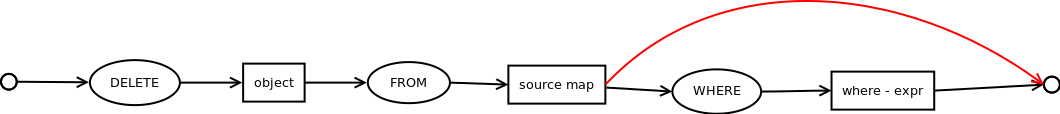
\includegraphics[scale=0.4]{images/delete}
		\caption{A DELETE lekérdezés szintaxis diagramja}
		\label{fig:deleteSytnax}
	\end{center}
\end{figure}

A szintaxis diagram alapján ezek a metódusok hívódnak meg a DeleteBuilder objektumnak:

DeleteBuilder builder = new Builder(); \\
builder.createDelete("mine"); \\ 
builder.setFrom("azeroth"); \\
builder.addOperandPiece("mine.x"); \\
builder.addOperator(">"); \\
builder.addOperandPiece("10"); \\
builder.build(); \\

Minden builder osztályban definiáltunk egy build metódust, ami egy IQueryObject példányt ad vissza. Minden lekérdezés objektum implementálja az IQueryObject interfészt, ami egy execute() metódust tartalmaz.



\section{ALTER lekérdezés felépítése}

A következő lekérdezés érkezik az adatbázismotorhoz:
\begin{sql}
ALTER CLASS Rectangle DELETEATTRIBUTE x;
\end{sql}


\begin{figure}[htb]
	\begin{center}
		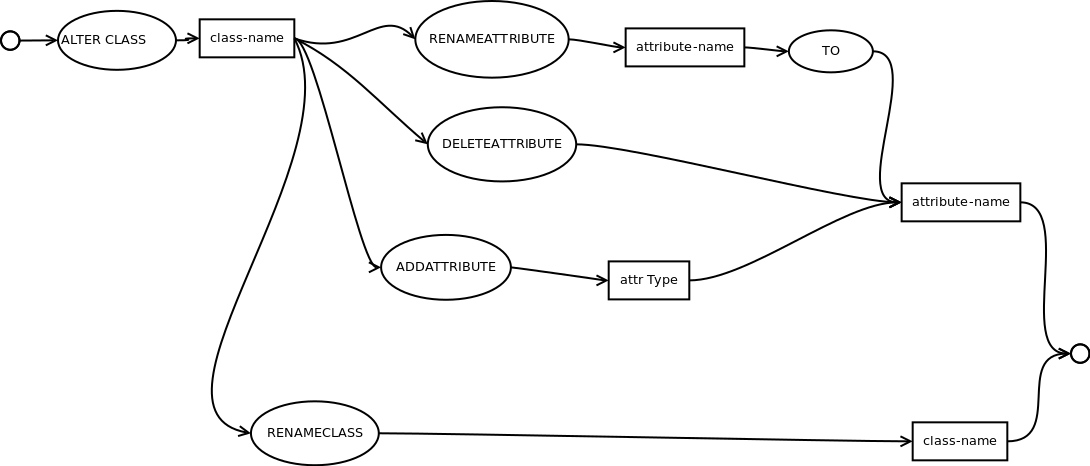
\includegraphics[scale=0.4]{images/alter}
		\caption{Az ALTER lekérdezés szintaxis diagramja}
		\label{fig:alterSytnax}
	\end{center}
\end{figure}

A builder objektum metódusainak használata a fenti lekérdezés esetében:

AlterBuilder builder = new AlterBuilder(); \\
builder.createAlter("Rectangle"); \\
builder.setAlterType("DELETEATTRIBUTE"); \\
builder.setStringAttribute("x"); \\
builder.build(); \\

Az Alter lekérdezés 4 típust definiál:

\begin{itemize}
\item Osztálynév módosítás
\item Attribútum törlés
\item Attribútum definiálás
\item Attribútum átnevezése
\end{itemize}

Ezek közül az attribútum létrehozáshoz és átnevezéshez egy plusz attribútumra van szükség, amelyet a builder.setOptionalValue(attribute-name or attribute-Type)
metódussal állíthatjuk be.

\section{CREATE lekérdezés felépítése}

A CREATE lekérdezéssel adatbázist, térképet és osztály definíciót lehet létrehozni. Az adatbázisnak és a térképnek a definiálása a legkönnyebb lekérdezések egyike, és az osztály definiálása ugyan azon lépésekből áll, csak egy párat definiál pluszba hozzájuk.

\begin{figure}[htb]
	\begin{center}
		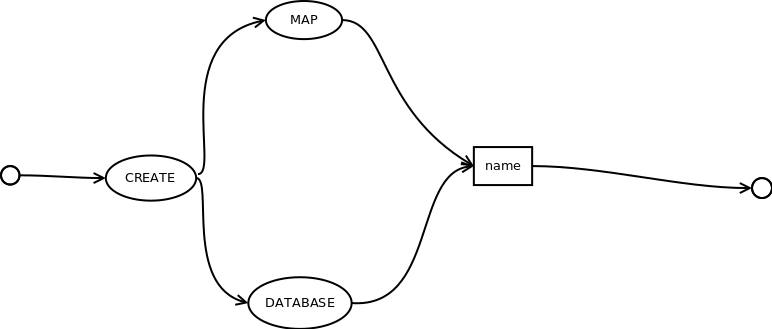
\includegraphics[scale=0.4]{images/create}
		\caption{A CREATE lekérdezés szintaxis diagramja adatbázis és térkép létrehozásra szűkítve}
		\label{fig:createSytnax}
	\end{center}
\end{figure}

\begin{figure}[htb]
	\begin{center}
		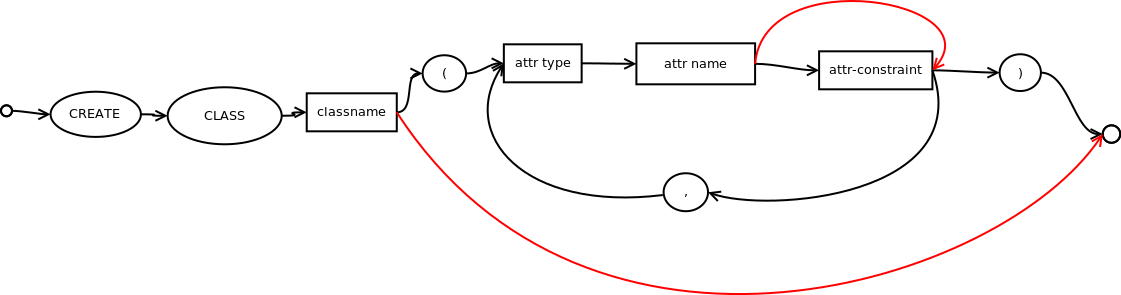
\includegraphics[scale=0.4]{images/createclass}
		\caption{A CREATE lekérdezés szintaxis diagramja osztálydefiníció definiálásához}
		\label{fig:createClassSytnax}
	\end{center}
\end{figure}



A következő lekérdezés érkezik az adatbázismotorhoz:
\begin{sql}
CREATE CLASS Harcos(
Number kor,
Number attack DEFAULT 10,
String nev);
\end{sql}

CreateBuilder builder = new CreateBuilder();
builder.setCreateType("CLASS"); \\
builder.setTheCommonValue("Harcos"); \\
builder.addAttributeParam("Number"); \\
builder.addAttributeParam("kor"); \\
builder.insertAttribute(); \\
builder.addAttributeParam("Number"); \\
builder.addAttributeParam("attack"); \\
builder.addAttributeParam("10"); \\
builder.insertAttribute(); \\
builder.addAttributeParam("String"); \\
builder.addAttributeParam("nev"); \\
builder.build(); \\

Vessző karaktereknél és a ")" karakternél hívódik meg az insertAttribute metódus, ami beszúrja az attribútumot.


\section{UPDATE lekérdezés felépítése}

A következő lekérdezés érkezik az adatbázismotorhoz:
\begin{sql}
UPDATE azeroth SET x=30,y=40 WHERE mine.id = 10;
\end{sql}

\begin{figure}[htb]
	\begin{center}
		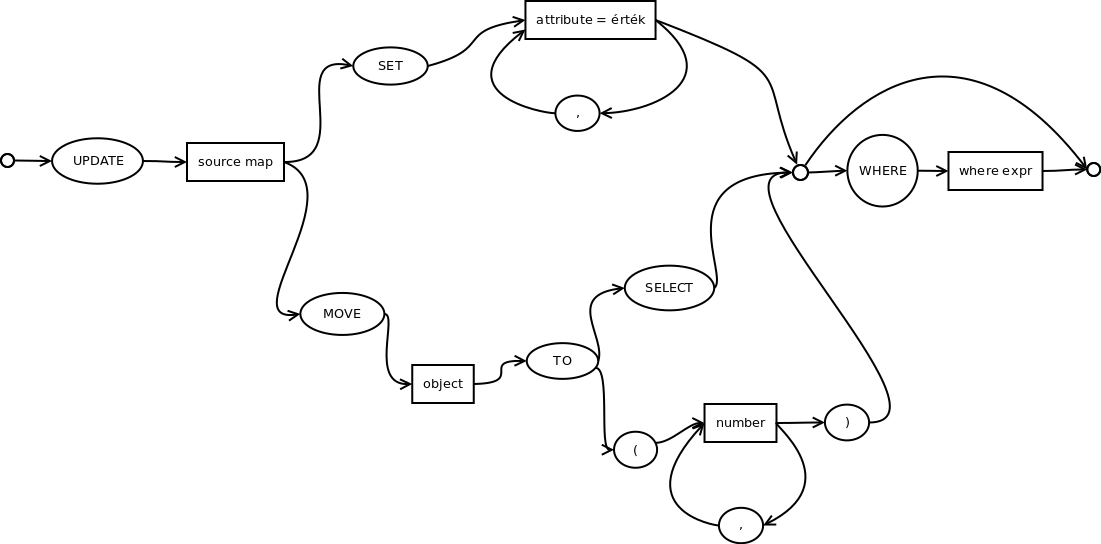
\includegraphics[scale=0.4]{images/update}
		\caption{Az UPDATE lekérdezés szintaxis diagramja}
		\label{fig:updateSytnax}
	\end{center}
\end{figure}



\section{Számítások optimalizálása}

Az adatbázismotor feladata levenni a terhet a felhasználó válláról, 
optimalizált algoritmusokkal támogatni a lekérdezéseket. Térképfelosztás, pályaelem összevonás, ezek mind olyan feladatok,
amelyek a térképműveletek gyorsabb végrehajtását idézik elő.
Mivel a dolgozatnak egyenlőre nem célja, hogy a piacon versenyképes szoftver legyen, ezért az optimalizálás nem került bele a dolgozatba.



\Chapter{Grafikus szerkesztőeszköz}

\section{Az editor funkciói}

\begin{itemize}
\item Admin felület: Ennek a grafikus felületnek az a célja, hogy az
adatbázissal kapcsolatos műveleteket grafikus felületen kezelhessük, nem pedig konzolos parancsok beírásával.
\item Térkép szerkesztő: Grafikus felületen összerakhatjuk a játékban szereplő térképet, és a háttérben ezeket a lekérdezéseket az editor adja ki.
\item Debug eszköz: Beírhatunk lekérdezéseket is a szerkesztőbe, és a lekérdezés eredményét rögtön láthatjuk is a térképen. Ha elemek kijelölése volt a lekérdezésben, akkor a térképen piros keretet rak az eredményhalmazban szereplő entitások köré.
	
\end{itemize}

\section{Implementáció}

A grafikus szerkesztőeszközt is Java nyelven implementáltam. Itt a szerkesztő az adatbázismotort könyvtárként foglalja magába. Az editor az egy egyszerű Swinges alkalmazásként lett megvalósítva. 

\section{Editor használati útmutató}

\begin{figure}[htb]
	\begin{center}
		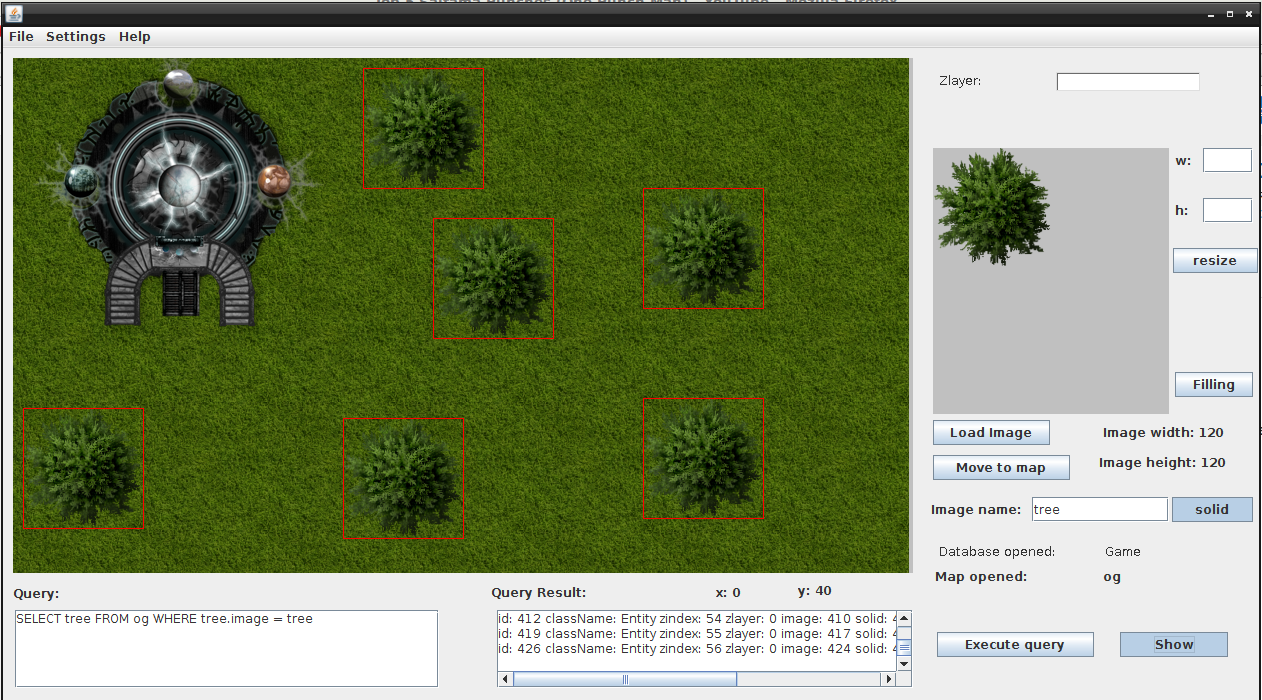
\includegraphics[scale=0.3]{images/editor}
		\caption{A Tile Editor használat közben}
		\label{fig:editor}
	\end{center}
\end{figure}

A File menü alatt hozható létre új adatbázis, azon belül új map, illetve létező adatbázis, és map is innen érhető el. Ez a menüpont tartalmaz még egy Save opciót is, ami arra szolgál, hogy a változtatásokat mentsük a JSOn fájlba. Ha módosítunk az adatbázison, de a Save menüt nem használjuk, akkor az editor kikapcsolása után a memóriából az összes változtatás eltűnik, és perzsiztens állapotról így nem gondoskodik.

Settings menü egyetlen funkciót tartalmaz, a Camera Settings beállítást, ami arra szolgál, hogy az irányító gombokkal(fel,le,jobbra,balra) hány pixelt ugorjon a kamera. Az alapértelmezett beállítás az, hogy az y tengely és az x tengely irányába is 10 pixellel mozdul el.
Ez azért fontos, mert nem lehet egérrel képeket beszúrni, hanem a "Move to Map" gombra kattintva szúr be egy képet a térképből látható terület bal felső sarkához igazítva. 

A Help menü alatt található egy rövid használati útmutató az alkalmazáshoz.

A főablak legnagyobb részét a térkép teszi ki, ahová beilleszthetünk képeket. Mellette a zlayer szövegdoboz arra szolgál, hogy egy számot írjunk bele, aminek akkor van jelentősége, amikor egy képet szúrunk a térképre, ugyanis ez a háttérben lefutó insert lekérdezésben a LAYER kulcsszó után szereplő attribútum. Ha ezt a mezőt nem töltjük ki, akkor sincs semmi probléma, olyankor a lekérdezés a háttérben automatikusan 0 értéket vesz fel a zlayernek.

A nagy térkép mellett látható egy kisebb téglalap is, amiben képek jelenhetnek meg. Ennek az a funkciója, hogy a beszúrandó képeket láthatjuk ott, illetve a mellette lévő két szövegdobozban(w, h) átméretezhetjük azt. 

A LoadImage gomb segítségével érhetjük el a fájlrendszert, és tölthetünk be onnan képet az imént említett dobozba.

Az ImageWidth és ImageHeight feliratok az aktuálisan betöltött kép attribútumai, ez az információ hasznos lehet, mert így a kamerát beállíthatjuk, hogy milyen mértékben mozduljon el felhasználói beavatkozásra, és a betöltött képet kényelmesebben szúrhatjuk be.

Ha a "Move to Map" gombra kattintunk, viszont az "Image Name" szövegdobozba nem adtuk meg a beszúrandó kép nevét, akkor az alkalmazás figyelmeztetni fog, hogy ezt tegyük meg. Amit abba a szövegdobozba írunk, az a beszúrandó Entity objektum image attribútumának lesz az értéke. 

A "solid" az egy JToogleButton, ami azt jelenti, hogy két állapota van, vagy lenyomva van, vagy alapértelmezetten. Ha nincs aktiválva, akkor a beszúrandó új Entity objektum solid attribútumának értéke false lesz, ha aktiválva van akkor true. Ez azért fontos mert az ütközésvizsgálat ezen attribútumra épül, ugyanis ha egy entitás nem solid, akkor az ütközésvizsgálat szempontjából semleges.

Az "Image Name" szövegdoboz alatt két felirat látható, amelyek az épp aktuálisan megnyitott adatbázis és map nevét mutatják. Ha megnyitjuk az editort akkor ezek értelem szerűen még nem tartalmaznak értéket, ezért ilyenkor a "-" karakter látható feltüntetve.

Az "Execute Query" gombra kattintva a "Query" Szövegmezőben látható lekérdezés fog lefutni, aminek eredménye a "Query Result:" szövegmezőben látható. Ha bekapcsolja a felhasználó a debug módot, akkor e térképen a lekérdezés eredményei láthatóvá válnak oly módon, hogy egy piros taglalap rajzolódik köré. A debig módot a show JToogleButton aktiválásával lehet bekapcsolni. 


\Chapter{Minta alkalmazás}

public static void main(String[] args) {
		InMemoryDatabase database = new InMemoryDatabase("Game");
		List<Instance> map = database.executeQuery("SELECT entity FROM og WHERE entity COLLIDE [1000,10]");
		
		for(int i=0;i<map.size();i++){
			if(map.get(i).className.equals("Entity")){
				System.out.println(map.get(i).getAttribute("x").getValue());
			}
		}
		database.executeQuery("ALTER CLASS Entity RENAMEATTRIBUTE x TO newx ");
		database.executeQuery("DELETE obj FROM og WHERE obj IS Entity");
		
		database.persist();
		
	}
	
A minta alkalmazáson látható, hogy kis mennyiségű kóddal kezelhető az adatbázis. Az InMemorydatabase osztály példányosításával megnyitja az adatbázismotor az aktuálisan kezelendő adatbázishoz tartozó JSON fájlt. Innentől kezdve nincs más dolgunk, mint az adatbázis objektum executeQuery metódusát meghívni, paraméterként a lekérdezés szövegláncot átadni neki. A lekérdezések visszatérhetnek eredmény listával, amely lista az Instance objektumra van tipizálva a Java driver implementációban. Ezen a listán végigiterálva az összes eredmény objektumot elérhetjük, annak getAttribute metódusával pedig lekérdezhetőek az attribútumaik.

Ha az adatbázismotor által nyújtott szolgáltatásokat magunknak szeretnénk implementálni, akkor az a példaalkalmazás kódjának a több százszorosát fogja eredményezni, nem is beszélve a fejlesztési időben felfedezhető különbségről. 
Először is gondoskodni kellene az adatok perzisztálásáról, majd   szolgáltatásokat implementálni annak kezelésére. Ezt követően az ütközés vizsgálat, távolság számítás, útvonal tervezés megvalósítása következne, amelyek nem triviális programozási feladatok. Ha mind ezekkel elkészülnénk, akkor még mindig elvégzendő feladat lenne a kliens alkalmazást összekötni az imént felsorolt implementációkkal. Könnyen belátható, hogy az elkészült adatbázismotor olyan eszköz, amely nélkülözhetetlen a játékfejlesztés folyamatában.



\Chapter{Összegzés}

A dolgozat keretein belül sikerült bebizonyítani, hogy szükség van térképadatbázisra kétdimenziós játékokhoz, amely a játéklogikát programozók számára lecsökkentheti a fejlesztési időt azzal, hogy kész eszközöket ad számára. Jelenleg az adatbázismotor nem tartalmaz optimalizált algoritmusokat, fő szempont a létjogosultság bizonyítása volt. A forráskódok elérhetőek GitHubon, így az interneten közzétéve lehetőség nyílik arra, hogy más játékfejlesztők igénybe vegyék, vagy teszteljék a szoftvert, észrevételeiket pedig eljuttassák hozzánk. Ahhoz, hogy a piacon versenyképes termék lehessen az adatbázismotorból, ahhoz még néhány funkciót implementálni kell, illetve optimalizált algoritmusokkal szeretném támogatni a szolgáltatásokat. Mivel jelenleg egyetlen kész eszközt sem implementáltak az adott probléma megoldására, amely ellátná az általunk kitalált és megvalósított adatbázismotor szolgáltatásait, ezért ha teljesen kész lesz a motor és a hozzá tartozó lekérdezőnyelv, akkor minden általam készített kétdimenziós játékban szeretném használni, és reményeim szerint nagyobb játékfejlesztő közösség is szívesen építené az alkalmazás logikáját az adatbázismotorra.


% \Chapter{Irodalomjegyzék}
\begin{thebibliography}{9}
\addcontentsline{toc}{chapter}{Irodalomjegyzék}
% \addcontentsline{toc}{chapter}{Irodalomjegyzék}

% http://books.google.de/books?hl=de&lr=&id=nEh4D4e88NwC&oi=fnd&pg=PA1&dq=Formal+Concept+Analysis+Fondations+and+Applications&ots=GSCkikE8pv&sig=8TJOPrSW07sJqLH0hF8_-HH_gb4#v=onepage&q=Formal%20Concept%20Analysis%20Fondations%20and%20Applications&f=false

% http://www.google.com/books?id=nEh4D4e88NwC&lpg=PA1&ots=GSFpjeHaqq&dq=bernhard%20ganter%20rudolf%20wille%20formal%20concept%20analysis%202004&lr&hl=hu&pg=PA2#v=onepage&q=bernhard%20ganter%20rudolf%20wille%20formal%20concept%20analysis%202004&f=false

\bibitem[AS09]{AS09}
Andrews, S.: \emph{In-Close, a fast algorithm for computing formal concepts},\\
International Conference on Conceptual Structures (ICCS),\\
Moscow, 2009.

\bibitem[KC10]{KC10}
Kristina Chodorow, Michael Dirolf: \emph{MongoDB: The Definitive Guide}, \\
O'Reilly Media, 2012.

\bibitem[GW05]{GW05}
Bernhard Ganter, Gerd Stumme, Rudolf Wille:\\
\emph{Formal Concept Analysis, Foundations and Applications},\\
Springer, 2005.

% http://link.springer.com/chapter/10.1007%2F978-3-540-78582-8_9#page-1
% http://www.palgrave-journals.com/kmrp/journal/v8/n3/full/kmrp201010a.html
\bibitem[KB08]{KB08}
Hak-Lae Kim, John G. Breslin, Sung-Kwon Yang, Hong-Gee Kim: \\
\emph{Social Semantic Cloud of Tag: Semantic Model for Social Tagging} \\
Springer-Verlag Berlin Heidelberg, 2008.

\bibitem[KL07]{KL07}
Kovács László: \emph{Generating Decision Tree from Lattice for Classification}, \\
Proceeding of ICAI07, Eger, 2007, 377-385.

\bibitem[KA08]{KA08}
Körei Attila: \textit{Fogalomhálók alkalmazása osztályfelbontási problémákra}, \\
PhD értekezés, Miskolci Egyetem, 2008.

% http://dl.acm.org/citation.cfm?id=321481
\bibitem[DM68]{DM68}
Donald R. Morrison: \\
\textit{PATRICIA - Practical Algorithm To Retrieve Information Coded in Alphanumeric}, \\
Journal of the ACM, Volume 15 Issue 4, Oct. 1968.

\bibitem[PP08]{PP08}
Alexandre Passant, Philippe Laublet: \emph{Meaning Of A Tag: A Collaborative Approach to Bridge the Gap Between Tagging and Linked Data} \\
Université Paris-Sorbonne, 2008.

\bibitem[RS98]{RS98}
Radeleczki, S.: \emph{A fogalomhálók egy műszaki alkalmazása}, \\
International Conference on Computer Science, "MicroCAD'98", \\
Section Applied Mathematics, University of Miskolc, March 12., 1998. pp. 1-7.

\bibitem[RR04]{RR04}
Rusty Russel, Daniel Quinlan, Christopher Yeoh: \\
\emph{Filesystem Hierarchy Standard}, \\
Filesystem Hierarchy Standard Group, 2004.

\bibitem[SF12]{SF12}
Steve Francia: \emph{MongoDB and PHP}, \\
O'Reilly Media, 2012.

\bibitem[SS06]{SS06}
Simon Schenk, Olaf Görlitz, Steffen Staab: \\
\emph{TagFS: Bringing Semantic Metadata to the Filesystem}, \\
Institute for Computer Science, University of Koblenz, 2006.

\newpage

% ================================================
\noindent {\huge \textbf{Internetes hivatkozások}}

\bigskip

\bibitem[BL98]{BL98}
Tim Berners-Lee: \textit{Semantic Web Road map}, \\
\texttt{http://www.w3.org/DesignIssues/Semantic.html} \\
Internet, 2013.

\bibitem[Elyse]{Elyse}
Silkwood Software: \emph{Elyse, freedom from folders}, \\
\texttt{http://silkwoodsoftware.com} \\
Internet, 2013.

\bibitem[Nepomuk]{Nepomuk}
\emph{Networked Environment for Personalized, \\
Ontology-based Management of Unified Knowledge}, \\
\texttt{http://nepomuk.kde.org} \\
Internet, 2013.

\bibitem[Referencer]{Referencer}
Referencer, GNOME Document Organiser \\
\texttt{https://launchpad.net/referencer} \\
Internet, 2013.

\bibitem[SpotLight]{SpotLight}
Apple: \textit{OS X. It's what a Mac a Mac} \\
\texttt{http://www.apple.com/osx/what-is} \\
Internet, 2013.

\bibitem[Tabbles]{Tabbles}
Yellow Blue Soft: \emph{Tabbles, folders evolved}, \\
\texttt{http://tabbles.net} \\
Internet, 2013.

\bibitem[Tag2find]{Tag2find}
\emph{Tag2find, Tag everything on your desktop}, \\
\texttt{http://www.tag2find.com} \\
Internet, 2013.

\bibitem[TaggedFrog]{TaggedFrog}
LunarFrog Software: \emph{TaggedFrog}, \\
\texttt{http://lunarfrog.com/taggedfrog} \\
Internet, 2013.

\bibitem[Tagsistant]{Tagsistant}
Tagsistant, All your files, quickly and easily. \\
\texttt{http://www.tagsistant.net} \\
Internet, 2013.

\bibitem[Tracker]{Tracker}
\texttt{https://live.gnome.org/Tracker} \\
GNOME (Meta) Tracker \\
Internet, 2013.

\bibitem[WinFS]{WinFS}
WinFS Team Blog \\
\texttt{http://blogs.msdn.com/b/winfs} \\
Internet, 2013.

\end{thebibliography}

 % 2

\end{document}

